\chapter{Methodik}
\label{cha:Methodik}

\section{Formulierung als Markov-Entscheidungsprozess}
\label{sec:meth_mdp}

Die autonome Drohnenlandung in einem vertikalen Korridor mit Hindernissen wird
als endlicher, episodischer Markov-Entscheidungsprozess (MDP) formalisiert
(vgl.\ Abschnitt~\ref{subsec:mdp}). Das MDP ist durch das Tupel
$(\mathcal{S}, \mathcal{A}, p, r, \gamma)$ definiert, wobei $\mathcal{S}$ den
Zustandsraum, $\mathcal{A}$ den Aktionsraum, $p$ die Übergangsdynamik, $r$ die
Belohnungsfunktion und $\gamma = 0{,}99$ den Diskontierungsfaktor bezeichnen.

\subsection{Zustandsraum}
\label{subsec:meth_zustandsraum}

Der Zustand $s_t \in \mathcal{S}$ zum Entscheidungszeitpunkt~$t$ setzt sich aus
einem numerischen Zustandsvektor $\mathbf{o}_t \in \mathbb{R}^{17}$ und einem
Tiefenbild $\mathbf{D}_t \in [0,1]^{64 \times 64}$ zusammen:
\begin{equation} \label{eq:meth_state}
  s_t = \bigl(\mathbf{o}_t,\;\mathbf{D}_t\bigr).
\end{equation}

Der Zustandsvektor
\begin{equation} \label{eq:meth_obs_vector}
  \mathbf{o}_t = \bigl(\,\tilde{\mathbf{p}}_{\mathrm{rel},t},\;\;
  \mathbf{q}_t,\;\;
  \tilde{\mathbf{v}}_t^{\,B},\;\;
  \tilde{\boldsymbol{\omega}}_t^{\,B},\;\;
  \mathbf{a}_{t-1}\,\bigr)
\end{equation}
enthält die in Tabelle~\ref{tab:meth_obs} aufgeschlüsselten Größen. Die Tilde
kennzeichnet skalierte und auf $[-1,1]$ geklippte Werte; die
Skalierungsfaktoren normieren die physikalischen Bereiche auf eine einheitliche
Größenordnung.

\begin{table}[ht]
\centering
\caption{Komponenten des Zustandsvektors $\mathbf{o}_t \in \mathbb{R}^{17}$.}
\label{tab:meth_obs}
\small
\begin{tabular}{l c l c}
\toprule
\textbf{Größe} & \textbf{Dim.} & \textbf{Beschreibung} & \textbf{Skalierung} \\
\midrule
$\tilde{\mathbf{p}}_{\mathrm{rel},t}$ & $3$ & Relative Position zum Ziel
  & $\times\tfrac{1}{15}$, ${\in}\,[-1,1]$ \\[2pt]
$\mathbf{q}_t$ & $4$ & Orientierungsquaternion $(w,x,y,z)$ & --- \\[2pt]
$\tilde{\mathbf{v}}_t^{\,B}$ & $3$ & Lineargeschwindigkeit
  & $\times\,0{,}4$, ${\in}\,[-1,1]$ \\[2pt]
$\tilde{\boldsymbol{\omega}}_t^{\,B}$ & $3$ & Winkelgeschwindigkeit
  & $\times\tfrac{1}{\pi}$, ${\in}\,[-1,1]$ \\[2pt]
$\mathbf{a}_{t-1}$ & $4$ & Aktion des vorherigen Zeitschritts & --- \\
\bottomrule
\end{tabular}
\end{table}

Die relative Position
$\tilde{\mathbf{p}}_{\mathrm{rel},t} =
\min\!\bigl(\max\!\bigl(\tfrac{1}{15}(\mathbf{p}_{\mathrm{ziel}} -
\mathbf{p}_t),\; -1\bigr),\; 1\bigr)$
kodiert Abstand und Richtung zum Landeziel, wobei der Skalierungsfaktor auf die
maximale Diagonaldistanz zum Ziel ausgelegt ist. Die Lineargeschwindigkeit wird
mit dem Faktor~$0{,}4$ skaliert, sodass der typische Geschwindigkeitsbereich der
Drohne auf $[-1,1]$ abgebildet wird; die Winkelgeschwindigkeit wird durch~$\pi$
dividiert und erreicht damit bei einer vollen Drehung pro Sekunde den
Sättigungswert.

Das Tiefenbild $\mathbf{D}_t \in [0,1]^{64 \times 64}$ wird von einer am
Drohnenkörper vertikal nach unten gerichteten Kamera mit $90^{\circ}$~Sichtfeld
erzeugt:
\begin{equation} \label{eq:meth_depth}
  \mathbf{D}_t = \min\!\left(\max\!\left(\frac{\mathbf{d}_{\mathrm{roh}}}{d_{\max}},
  \; 0\right),\; 1\right), \quad d_{\max} = 20\,\text{m}.
\end{equation}
Das Tiefenbild liefert die einzige Information über Lage und Geometrie der
Hindernisse; der numerische Zustandsvektor enthält keine explizite
Hindernisrepräsentation.

\subsection{Aktionsraum}
\label{subsec:meth_aktionsraum}

Der Aktionsraum ist vierdimensional und kontinuierlich:
\begin{equation} \label{eq:meth_action}
  \mathbf{a}_t = (a_x,\; a_y,\; a_z,\; a_\psi) \in [-1,\; 1]^4.
\end{equation}
Die ersten drei Komponenten definieren einen Positionsversatz relativ zur aktuellen
Drohnenposition:
\begin{equation} \label{eq:meth_target_pos}
  \mathbf{p}_{\mathrm{soll}} = \mathbf{p}_t +
  \begin{pmatrix} a_x \cdot \sigma_x \\ a_y \cdot \sigma_y \\ a_z \cdot \sigma_z \end{pmatrix},
  \quad \boldsymbol{\sigma} = (1{,}0;\; 1{,}0;\; 2{,}0)\,\text{m}.
\end{equation}
Die erhöhte $z$-Skala ermöglicht größere vertikale Schritte, die für den
vorwiegend vertikalen Abstieg erforderlich sind. Die vierte Komponente legt den
Sollgierwinkel fest:
\begin{equation} \label{eq:meth_target_yaw}
  \psi_{\mathrm{soll}} = a_\psi \cdot 180^{\circ}.
\end{equation}

Die Sollwerte $(\mathbf{p}_{\mathrm{soll}}, \psi_{\mathrm{soll}})$ werden
nicht direkt an die Motoren übergeben, sondern von einem kaskadierenden
PID-Regler in Motordrehzahlen umgesetzt
(vgl.\ Abschnitt~\ref{subsec:meth_uebergangsmodell}). Diese Entkopplung
reduziert den Aktionsraum von vier Motordrehzahlen auf vier semantisch
interpretierbare Navigationskommandos.

\subsection{Übergangsmodell}
\label{subsec:meth_uebergangsmodell}

Die Übergangsdynamik $p(s_{t+1} \mid s_t, \mathbf{a}_t)$ wird deterministisch
durch den Physiksimulator bestimmt. Der Simulator integriert die Physik mit
einer Schrittweite von $\Delta t = 0{,}01$\,s (100\,Hz). Der RL-Agent trifft
nicht bei jedem Simulationsschritt eine Entscheidung, sondern alle
300~Schritte, entsprechend einem Entscheidungsintervall von $3{,}0$\,s. Zwischen
zwei Entscheidungen steuert ein kaskadierender PID-Regler die Drohne zum
Sollzustand $(\mathbf{p}_{\mathrm{soll}}, \psi_{\mathrm{soll}})$.

\subsection{Belohnungsfunktion}
\label{subsec:meth_belohnung}

Die Belohnungsstruktur kombiniert dichte Belohnungssignale mit spärlichen terminalen
Signalen, sie setzt sich als gewichtete Summe aus fünf Komponenten zusammen:
\begin{equation} \label{eq:meth_reward}
  r_t =\;
    w_{\mathrm{prog}}\, r_{\mathrm{prog}}
  + w_{\mathrm{nah}}\, r_{\mathrm{nah}}
  + w_{\mathrm{prox}}\, r_{\mathrm{prox}}
  + w_{\mathrm{crash}}\, r_{\mathrm{crash}}
  + w_{\mathrm{erf}}\, r_{\mathrm{erf}}
\end{equation}


\noindent\textbf{Fortschritt} ($w_{\mathrm{prog}} = 1{,}0$).\enspace
Die Fortschrittsbelohnung misst die Annäherung an das Ziel zwischen zwei
aufeinanderfolgenden Zeitschritten:
\begin{equation}
  r_{\mathrm{prog}} = d_t - d_{t+1}.
\end{equation}
Dabei bezeichnet $d_t = \lVert\mathbf{p}_{\mathrm{ziel}} - \mathbf{p}_t\rVert$
den euklidischen Abstand zum Ziel.
Ein positiver Wert zeigt an, dass sich die Drohne dem Ziel genähert hat.

\noindent\textbf{Nähe} ($w_{\mathrm{nah}} = 2{,}0$).\enspace
Die Nähebelohnung liefert ein exponentiell ansteigendes Signal, pro Zeitschritt im Nahbereich
des Ziels:
\begin{equation}
  r_{\mathrm{nah}} = \exp(-d_{t+1}).
\end{equation}
Bei Abständen über ca.\ 3\,m ist $r_{\mathrm{nah}} \approx 0$; am Ziel nähert
sich der Wert~$1$.

\noindent\textbf{Hindernisproximität} ($w_{\mathrm{prox}} = -0{,}2$).\enspace
Die Hindernisproximität bestraft das Eindringen in einen Sicherheitsradius
$d_{\mathrm{s}} = 3{,}0$\,m um Hindernisse:
\begin{equation}
  r_{\mathrm{prox}} = \max\!\left(1 - \frac{d_{\mathrm{min}}}{d_{\mathrm{s}}},\; 0\right),
\end{equation}
wobei $d_{\mathrm{min}}$ den minimalen Abstand zur achsenparallelen
Begrenzungsbox (AABB) des nächsten Hindernisses bezeichnet. Die Strafe steigt
linear mit abnehmendem Abstand.

\noindent\textbf{Absturz} ($w_{\mathrm{crash}} = -10{,}0$).\enspace
Die Absturzstrafe wird bei Verletzung einer Abbruchbedingung
(vgl.\ Abschnitt~\ref{subsec:meth_terminierung}) ausgelöst:
\begin{equation}
  r_{\mathrm{crash}} =
  \begin{cases}
    1 & \text{Hinderniskollision, Bodenkollision, Kontrollverlust} \\
      & \text{oder Verlassen des Korridors,} \\
    0 & \text{sonst.}
  \end{cases}
\end{equation}

\noindent\textbf{Erfolg} ($w_{\mathrm{erf}} = 20{,}0$).\enspace
Der Erfolgsbonus wird bei Erreichen des Landeziels vergeben:
\begin{equation}
  r_{\mathrm{erf}} =
  \begin{cases}
    1 & \text{Landung innerhalb des Zielradius,} \\
    0 & \text{sonst.}
  \end{cases}
\end{equation}

\section{Netzwerkarchitektur}
\label{sec:meth_architektur}

PPO verwendet eine Actor-Critic-Architektur
(vgl.\ Abschnitt~\ref{subsec:ppo_clip}), in der zwei Netzwerke parallel
trainiert werden: Der \emph{Actor}~$\pi_\theta$ gibt eine stochastische
Strategie aus, der \emph{Critic}~$V_\phi$ schätzt die State-Value-Funktion zur
Berechnung des Vorteilsschätzers.

Der CNN-Encoder besteht aus drei Faltungsschichten mit aufsteigender Kanalzahl
(32, 64, 128), abnehmenden Kernelgrößen ($8 \times 8$, $4 \times 4$,
$3 \times 3$) und Schrittweiten (4, 2, 1). Nach jeder Faltungsschicht folgt
eine Batch-Normalisierung und eine ELU-Aktivierung. Ein abschließendes Global
Max Pooling reduziert jede der 128~Feature-Maps auf einen Skalar und erzeugt so
einen 128-dimensionalen Merkmalsvektor unabhängig von der räumlichen Auflösung
der Eingabe. Der Zustandsvektor durchläuft vor der Konkatenation eine laufende
empirische Normalisierung, die Mittelwert und Varianz über alle bisherigen
Beobachtungen schätzt und die heterogenen physikalischen Größen auf einheitliche
Skala bringt. Der resultierende Vektor aus CNN-Merkmalen und normalisiertem
Zustand wird an die MLP-Köpfe von Actor und Critic weitergegeben, die jeweils
aus drei vollvernetzten Schichten mit 128~Neuronen und ELU-Aktivierung bestehen.
Actor und Critic teilen sich den CNN-Encoder; die MLP-Köpfe werden getrennt
trainiert. Der Actor gibt pro Aktionsdimension einen Mittelwert~$\mu$ und eine
lernbare Log-Standardabweichung $\log\sigma$ aus und parametrisiert damit eine
Tanh-Gaußverteilung, deren Motivation und Formulierung in
Abschnitt~\ref{subsubsec:meth_tanh_squashing} erläutert werden. Der Critic
gibt einen skalaren State-Value $V(s_t)$ aus.
Abbildung~\ref{fig:meth_architecture} zeigt die vollständige Architektur mit
allen Schichten.

\begin{figure}[ht]
    \centering
    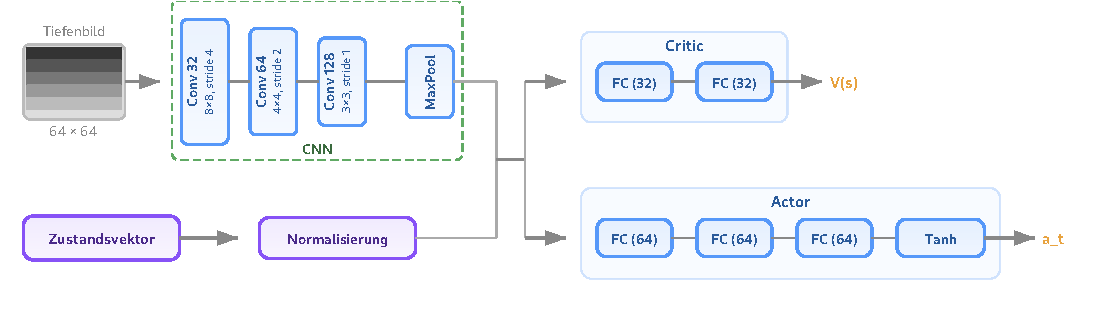
\includegraphics[width=\linewidth]{Bilder/architecture.pdf}
    \caption{Netzwerkarchitektur: Das Tiefenbild durchläuft einen geteilten
    CNN-Encoder (drei Faltungsschichten mit Batch-Normalisierung, ELU und
    abschließendem Global Max Pooling). Der resultierende 128-dimensionale
    Merkmalsvektor wird mit dem empirisch normalisierten Zustandsvektor
    konkateniert und an die getrennten MLP-Köpfe von Actor und Critic
    weitergegeben.}
    \label{fig:meth_architecture}
\end{figure}

\section{Trainingsverfahren}
\label{sec:meth_trainingsverfahren}

\subsection{Proximal Policy Optimization}
\label{subsec:meth_ppo}

Als Trainingsalgorithmus wird \emph{Proximal Policy Optimization} (PPO)
\autocite{schulmanProximalPolicyOptimization2017} eingesetzt, dessen Clipped Surrogate
Objective und vollständige Zielfunktion in Abschnitt~\ref{subsec:ppo_clip} eingeführt
wurden.

Die vorliegende Arbeit zielt auf einen kontinuierlichen Aktionsraum ab, in dem der Agent
Zielpositionsoffsets und eine Gierrate ausgibt (vgl.\
Abschnitt~\ref{subsec:meth_aktionsraum}). Wie in Abschnitt~\ref{subsec:ppo_clip} dargelegt,
übertrifft PPO auf strukturell vergleichbaren kontinuierlichen Steuerungsaufgaben die
Vergleichsverfahren TRPO und A2C. Auch im spezifischen
Anwendungsfeld der Drohnensteuerung hat sich PPO als Standardverfahren etabliert: Sowohl
\textcite{bartolomeiAutonomousEmergencyLanding2022} und
\textcite{xuNavRLLearningSafe2024} als auch
\textcite{kaufmannChampionlevelDroneRacing2023} setzen PPO ein
(vgl.\ Abschnitt~\ref{sec:architektur}). 
PPO passt zudem architektonisch zum gewählten
Trainingssetup: Als On-Policy-Verfahren verarbeitet es die gesammelten Daten direkt und
verwirft sie nach dem Update. Off-Policy-Verfahren wie SAC
\autocite{haarnojaOffPolicyMaximumEntropy2017} wurden daher verworfen. Sie erfordern
einen Replay Buffer, der vergangene Transitionen speichert und bei jedem Update erneut
abtastet. Ihre höhere Sample-Effizienz setzt zudem voraus, dass die Datensammlung der
Engpass ist. Bei GPU-paralleler Simulation mit hunderten bis tausenden Umgebungen ist
jedoch der Gradientenupdate der Engpass; die geringere Sample-Effizienz von
On-Policy-Methoden wird durch den Datendurchsatz mehr als kompensiert
\autocite{rudinLearningWalkMinutes2022}. Zudem würde ein Replay Buffer Transitionen aus
früheren Curriculum-Stufen enthalten (vgl.\
Abschnitt~\ref{subsec:meth_curriculum}), die für die aktuelle Stufe nicht mehr
repräsentativ sind.
Neuere PPO-Varianten wie Phasic Policy Gradient
\autocite{cobbePhrasicPolicyGradient2021} wurden nicht evaluiert, da die verwendete
Trainingsumgebung rsl-rl \autocite{rudinLearningWalkMinutes2022} ausschließlich die
Standard-PPO-Implementierung bereitstellt.

\subsubsection{Aktionsverteilung und Tanh-Squashing}
\label{subsubsec:meth_tanh_squashing}

Der Actor parametrisiert eine Gaußverteilung über einem unbeschränkten
Hilfsraum: Für jede Aktionsdimension~$i$ wird ein Rohwert
$u_i \sim \mathcal{N}(\mu_i, \sigma_i^2)$ gesampelt, wobei~$\mu_i$ und
$\log\sigma_i$ Netzausgaben sind. Der Aktionsraum ist jedoch auf $[-1,1]^4$
beschränkt (vgl.\ Abschnitt~\ref{subsec:meth_aktionsraum}). Ein naives
Clipping $a_i = \mathrm{clip}(u_i, -1, 1)$ würde die Aktionswerte korrekt
begrenzen, die zugehörige Log-Wahrscheinlichkeit jedoch weiterhin auf dem
unbeschnittenen Wert~$u_i$ berechnen. Da PPO das Verhältnis
$r_t(\theta) = \pi_\theta(\mathbf{a}_t \mid s_t) \,/\,
\pi_{\theta_{\mathrm{alt}}}(\mathbf{a}_t \mid s_t)$ zur Gradientenschätzung
nutzt (vgl.\ Abschnitt~\ref{subsec:ppo_clip}), führt diese Diskrepanz
zwischen ausgeführter und bewerteter Aktion zu verzerrten Gradienten.

Statt Clipping wird daher eine invertierbare, differenzierbare Transformation
verwendet~\autocite{haarnojaOffPolicyMaximumEntropy2017}:
\begin{equation} \label{eq:meth_tanh_squashing}
  a_i = \tanh(u_i).
\end{equation}
Die zugehörige Log-Wahrscheinlichkeit ergibt sich über die
Substitutionsregel für Wahrscheinlichkeitsdichten (Change of Variables):
\begin{equation} \label{eq:meth_tanh_logprob}
  \log\pi(\mathbf{a} \mid s)
  = \log\mathcal{N}(\mathbf{u} \mid \boldsymbol{\mu}, \boldsymbol{\sigma}^2)
  - \sum_{i=1}^{4} \log\!\bigl(1 - \tanh^2(u_i)\bigr).
\end{equation}
Der Korrekturterm~$-\sum_i \log(1 - \tanh^2(u_i))$ ist die
Log-Jacobi-Determinante der Tanh-Transformation und stellt sicher, dass die
Dichte im transformierten Raum korrekt normiert bleibt.

Zusätzlich erzwingt ein Floor $\log\sigma_i \geq -2{,}0$
($\sigma_i \geq 0{,}135$) eine Mindestexploration. Ohne diesen Floor kann PPO
die Standardabweichung gegen null treiben, was in der Log-Wahrscheinlichkeit zu
numerischen Instabilitäten führt und die Strategie irreversibel kollabieren
lässt.

\subsubsection{Hyperparameter}
\label{subsubsec:meth_hyperparams}

Tabelle~\ref{tab:meth_ppo_hyperparams} fasst die PPO-Hyperparameter zusammen.

\begin{table}[ht]
\centering
\caption{PPO-Hyperparameter der vorliegenden Arbeit.}
\label{tab:meth_ppo_hyperparams}
\small
\begin{tabular}{l l}
\toprule
\textbf{Parameter} & \textbf{Wert} \\
\midrule
Clipping $\varepsilon$      & $0{,}2$ \\
Diskontierung $\gamma$      & $0{,}99$ \\
GAE $\lambda$               & $0{,}95$ \\
Lernrate $\alpha$           & $5 \times 10^{-4}$ \\
Lern-Epochen $K$            & $5$ \\
Mini-Batches $M$            & $4$ \\
$c_1$ (Value-Loss)          & $1{,}0$ \\
$c_2$ (Entropie)            & $0{,}003$ \\
Gradient-Clipping           & $1{,}0$ \\
Schritte pro Env $T$        & $60$ \\
Parallele Envs $N$          & $256$ \\
Optimizer                   & Adam \\
\bottomrule
\end{tabular}
\end{table}

Die Werte für $\varepsilon$, $\gamma$, $\lambda$ sowie $K$ und
Gradient-Clipping entsprechen den von
\textcite{schulmanProximalPolicyOptimization2017} empfohlenen Standardwerten, die sich
in den MuJoCo-Benchmarks als robust über verschiedene Aufgaben erwiesen haben.
Der GAE-Parameter $\lambda = 0{,}95$ folgt der Empfehlung von
\textcite{schulmanHighDimensionalContinuousControl2016} als Kompromiss zwischen Bias und
Varianz. Die Lernrate $\alpha = 5 \times 10^{-4}$ wurde experimentell bestimmt:
Kleinere Werte führten zu sehr langsamer Konvergenz, größere zu kollabierenden
Strategien. Aufgabenspezifisch angepasst wurden ferner die Rollout-Länge~$T$ — 60~Entscheidungen
bei 3\,s Entscheidungsintervall ergeben 180\,s Rollout-Dauer — sowie die Anzahl
paralleler Umgebungen $N = 256$, begrenzt durch den GPU-Speicher der verwendeten
NVIDIA~A30 (24\,GB). Der Entropie-Koeffizient~$c_2 = 0{,}003$ wurde bewusst niedrig
gewählt, da die Tanh-Verteilung
(vgl.\ Abschnitt~\ref{subsubsec:meth_tanh_squashing}) empfindlich auf hohe Entropie-Anreize reagiert;
$c_2 \geq 0{,}01$ führte in Pilotexperimenten zu instabilem Training.

\section{Trainingsumgebung}
\label{sec:meth_trainingsumgebung}

\subsection{Physiksimulator}
\label{subsec:meth_simulator}

Das Training eines RL-Agenten vorliegende Aufgabe erfordert einen
Physiksimulator, der drei zentrale Anforderungen erfüllt:
(1)~GPU-parallelisierte Ausführung hunderter Umgebungsinstanzen, um die von PPO
benötigten großen Rollout-Batches effizient zu erzeugen
(vgl.\ Abschnitt~\ref{sec:meth_trainingsverfahren});
(2)~simulierte Tiefenkameras, da der Agent Tiefenbilder als Beobachtung erhält;
(3)~Import beliebiger 3D-Objekte, um realitätsnahe Hindernisszenarien zu
konstruieren.

Die vorliegende Arbeit verwendet Genesis
\autocite{xianGenesisUniversalGenerative2024}, einen 2024 veröffentlichten,
quelloffenen Physiksimulator für Robotik. Genesis erfüllt alle drei definierten
Anforderungen: Der Simulator führt bis zu 4096~Umgebungen GPU-parallel aus,
stellt Tiefenkameras über eine Batch-Rendering-Pipeline bereit, importiert
beliebige 3D-Meshes (u.\,a.\ URDF, OBJ) und bietet eine durchgängige
Python-API. Genesis zeichnet sich durch eine geringere Einstiegskomplexität aus:
Die Installation beschränkt sich auf ein einzelnes Python-Paket, und die API
erfordert keine herstellerspezifische Toolchain.

Gegenüber verbreiteten Alternativen bietet Genesis entscheidende Vorteile:
Gazebo \autocite{koenigDesignUseParadigms2004} und PyBullet
\autocite{coumansPybulletPythonModule2016} unterstützen keine GPU-parallele
Ausführung hunderter Umgebungen und scheiden daher für datenintensives
RL-Training aus. Isaac Gym \autocite{makoviychukIsaacGymHigh2021} erfüllt zwar
alle genannten Anforderungen, ist jedoch proprietär an NVIDIA gebunden und
erfordert einen umfangreichen Installationsstack.

Einschränkend ist anzumerken, dass Genesis mit seiner Erstveröffentlichung im
Dezember~2024 ein vergleichsweise junges Projekt ist und über eine kleinere
Community als etablierte Alternativen verfügt.

\subsection{Drohnenmodell}
\label{subsec:meth_drohne}

Die Drohne wird als URDF-Modell mit vier Rotoren simuliert. Die wesentlichen
physikalischen Parameter sind eine Masse von $0{,}714$\,kg, ein
Schub-Gewicht-Verhältnis von $2{,}25$ sowie eine Hover-Drehzahl von
$1789$\,RPM bei einer maximalen Drehzahl von $2700$\,RPM.

\subsection{Korridorgeometrie}
\label{subsec:meth_korridor}

Die Trainingsumgebung bildet einen vertikalen Korridor der Ausdehnung
$5 \times 2 \times 15$\,m ($x \times y \times z$) ab
(Abbildung~\ref{fig:meth_corridor}). Der Korridor besitzt keine physischen
Wände; stattdessen wird das Verlassen des Begrenzungsrahmens als Absturz
gewertet (vgl.\ Abschnitt~\ref{subsec:meth_terminierung}). Die Bodenebene
befindet sich bei $z = 0$\,m.

Die Drohne wird zu Episodenbeginn auf einer zufälligen Position im oberen
Korridorbereich bei $z = 12$\,m initialisiert, wobei die horizontale Position
gleichverteilt innerhalb von $\pm 1{,}5$\,m ($x$) bzw.\ $\pm 0{,}5$\,m ($y$)
um die Korridormitte variiert. Die Initialorientierung ist die Nulllage
(Quaternion $(1,0,0,0)$). Das Landeziel ist fixiert bei
$\mathbf{p}_{\mathrm{ziel}} = (0,\; 0,\; 1)^{\!\top}$\,m.

Während des Abstiegs durchquert die Drohne zwei horizontale Hindernisschichten
bei $z \approx 2$\,m und $z \approx 7$\,m
(vgl.\ Abschnitt~\ref{subsec:meth_hindernisse}).

\begin{figure}[ht]
    \centering
    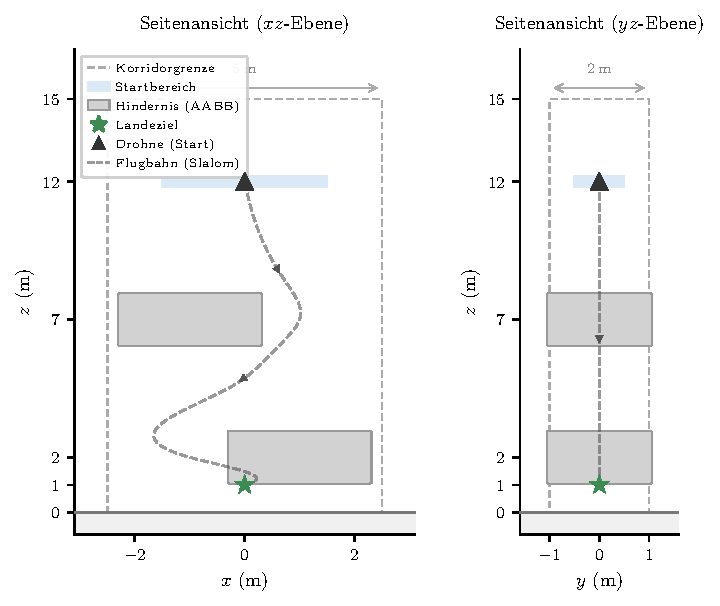
\includegraphics[width=0.85\linewidth]{Bilder/corridor_geometry.pdf}
    \caption{Seitenansichten der Korridorgeometrie. Links: $xz$-Ebene
    (Slalom-Achse) mit schematischer Flugbahn. Rechts: $yz$-Ebene. Die
    gestrichelten Rechtecke markieren die Korridorgrenzen, graue Flächen die
    schematischen Hindernis-Begrenzungsboxen.}
    \label{fig:meth_corridor}
\end{figure}

\subsection{Hindernisse}
\label{subsec:meth_hindernisse}

Als Hindernisse dienen sechs 3D-Objekte aus dem Google Scanned Objects
Datensatz~(GSO): eine Tasse, ein Teddybär, ein Spielzeugdinosaurier, ein
Spielzeugbus, ein Spielzeugnashorn und ein Schuh. Jedes Objekt wird um den
Faktor~$21$ bis~$63$ skaliert, sodass seine horizontale Ausdehnung mindestens
$2$\,m beträgt und damit die gesamte $y$-Breite des Korridors abdeckt. Objekte,
deren Höhe nach der Skalierung $2{,}0$\,m überschreitet, werden von unten
beschnitten.

Für die Kollisionserkennung und die Hindernisproximität
(vgl.\ Abschnitt~\ref{subsec:meth_belohnung}) wird die achsenparallele
Begrenzungsbox (AABB) jedes Objekts herangezogen. Diese konservative
Approximation umschließt das gesamte Mesh vollständig, sodass die Drohne
bereits vor Berührung der tatsächlichen Oberfläche als kollidiert gilt.

Die Platzierung folgt einem erzwungenen Slalom entlang der $x$-Achse: In jeder
der zwei Hindernisschichten wird ein zufällig gewähltes Objekt auf einer Seite
der Korridormitte positioniert, mit einem Versatz von $0{,}6$ bis $1{,}2$\,m.
Aufeinanderfolgende Schichten wechseln die Seite, sodass die Drohne einen
Slalomkurs fliegen muss. Die Startseite ($+x$ oder $-x$) wird pro Episode
zufällig gewählt.

\subsection{Verarbeitungspipeline}
\label{subsec:meth_pipeline}

Abbildung~\ref{fig:meth_pipeline} zeigt den vollständigen Datenfluss von der
Sensorik bis zur physikalischen Ausführung. Das normalisierte
Tiefenbild~$\mathbf{D}_t$ und der skalierte
Zustandsvektor~$\mathbf{o}_t$
(vgl.\ Abschnitt~\ref{subsec:meth_zustandsraum}) werden als
\texttt{TensorDict} gebündelt und der Actor-Critic-Architektur übergeben
(vgl.\ Abschnitt~\ref{sec:meth_architektur}). Die vom Actor gesampelte Aktion
wird gemäß Abschnitt~\ref{subsec:meth_aktionsraum} in Sollposition und
Sollgierwinkel skaliert und vom kaskadierenden PID-Regler
(vgl.\ Abschnitt~\ref{subsec:meth_uebergangsmodell}) über das
Entscheidungsintervall in Motordrehzahlen umgesetzt.

Sowohl das Tiefenbild als auch der Zustandsvektor werden direkt und
unverrauscht aus der Simulation erhoben. In einer realen Anwendung wären die
Tiefenbilder durch Sensorrauschen, Reflexionen und Ausfälle beeinflusst, und
die Zustandsinformationen müssten aus verrauschten IMU- und GPS-Messungen
geschätzt werden. Diese Idealisierung begrenzt die unmittelbare
Übertragbarkeit der trainierten Strategie auf reale Hardware.

\begin{figure}[ht]
    \centering
    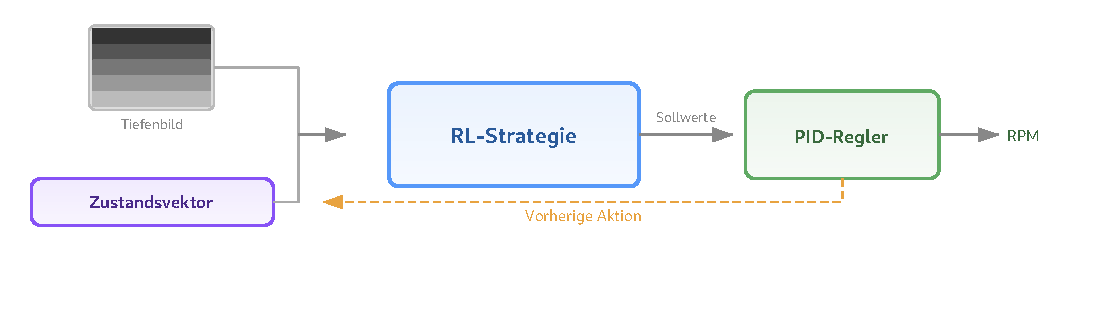
\includegraphics[width=\linewidth]{Bilder/pipeline.pdf}
    \caption{Verarbeitungspipeline: Tiefenbild und Zustandsvektor werden dem
    Actor-Netz (CNN~+~MLP) übergeben, das eine Aktion sampelt. Nach
    Skalierung steuert ein kaskadierender PID-Regler die Drohne über
    300~Simulationsschritte.}
    \label{fig:meth_pipeline}
\end{figure}

\subsection{Terminierung}
\label{subsec:meth_terminierung}

Eine Episode endet, wenn eine der folgenden Bedingungen eintritt:

\noindent\textbf{Erfolg.}\enspace Die Drohne verbleibt über die gesamte Dauer
eines Entscheidungsschritts ($3{,}0$\,s) innerhalb eines Radius von $0{,}5$\,m
um das Landeziel.

\noindent\textbf{Absturz.}\enspace Mindestens eine der folgenden Bedingungen
ist erfüllt:
\begin{itemize}
  \item Flughöhe $z < 0{,}2$\,m (Bodenkollision),
  \item Neigung $> 60^{\circ}$ in Roll oder Pitch (Kontrollverlust),
  \item AABB-Abstand zum nächsten Hindernis $< 0{,}3$\,m (Hinderniskollision),
  \item Verlassen des Korridors (Bounding-Box-Prüfung auf allen Achsen).
\end{itemize}

\noindent\textbf{Timeout.}\enspace Die maximale Episodenlänge von
$T_{\max} = 20$ Entscheidungsschritten ($60$\,s) ist erreicht. Timeouts werden
im Vorteilsschätzer als nicht-terminale Übergänge behandelt, sodass die
Wertfunktion den erwarteten Ertrag über die Episode hinaus approximiert.

\subsection{Curriculum}
\label{subsec:meth_curriculum}

Das Training folgt einem zweistufigen Curriculum. In der ersten Phase
(Iterationen~$0$ bis~$300$, entsprechend 18\,060~Entscheidungsschritten) sind
die Hindernisse deaktiviert, sodass der Agent zunächst den reinen Abstieg zum
Ziel erlernt. Die Korridorgrenzen sind von Beginn an aktiv. In der zweiten
Phase werden die Hindernisse bei jedem Episodenreset zufällig platziert und der
Agent muss sowohl die Navigation zum Ziel als auch die Hindernisvermeidung
bewältigen.